%!TEX root = ../thesis.tex
\section{Evaluation}
\label{kinectograph_study}

This section presents user feedback collected from three preliminary studies that we conducted to answer questions: What activities would users find useful to capture using Kinectograph? How well could users create self-directed tutorials with Kinectograph?

\subsection{Study 1: Demo at an Expo}
We demonstrated an initial design of Kinectograph (see Appendix C) at a public exhibition to approximately 60 people. Each participant was allowed to enter our capturing space and experience the device. Based on our observation and conversations collected, we found that people were convinced by the idea as soon as they walked into the scene when Kinectograph started to move along. These questions were often asked: \iquote{How fast was Kinectograph able to follow me?} and \iquote{Can I switch to track other parts (like my hand)?}. With the tablet device control, participants soon were successful in controlling the camera. They often walked, ran, and danced to test the tracking. We also learned that people expected the device to provide fast response in various conditions such as turning, rapid change of directions, or partial occlusions (when people were hidden by furniture or large objects).

\subsection{Study 2: Test on Recording Activities}
To understand how Kinectograph can support users in demonstrations, we invited four participants (3 male and 1 female, aged 22-29) who did not join the exhibition to our user study in a home environment. We aimed to explore whether users prefer to watch the video captured by Kinectograph over video recorded with a static camera, and whether Kinectograph can capture complete demonstrations
 that a static camera cannot achieve.

We first introduced Kinectograph by having participants walk around while the device tracked. We encouraged participants to brainstorm some activities they wanted to record. Once the task was decided, they were asked to set up both a static camera and the Kinectograph with our tablet device and start the recording. There was no time constraint during the study. A short post interview was then conducted, in which we showed the recorded videos from both cameras on a PC.

\begin{table}[b!]
     \centering
    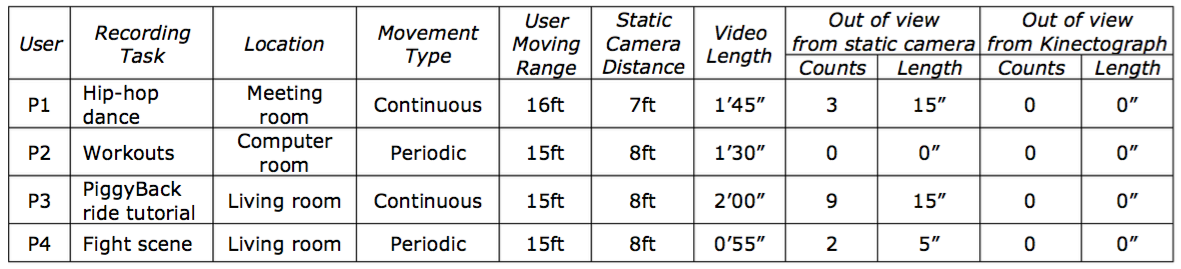
\includegraphics[width=1\columnwidth]{\kinectograph/fig/study2}
    \caption{Task information and results collected in the preliminary user study.}
    \label{tab:kinectograph_first_tasks}
 \end{table}

\begin{figure}[t!]
     \centering
    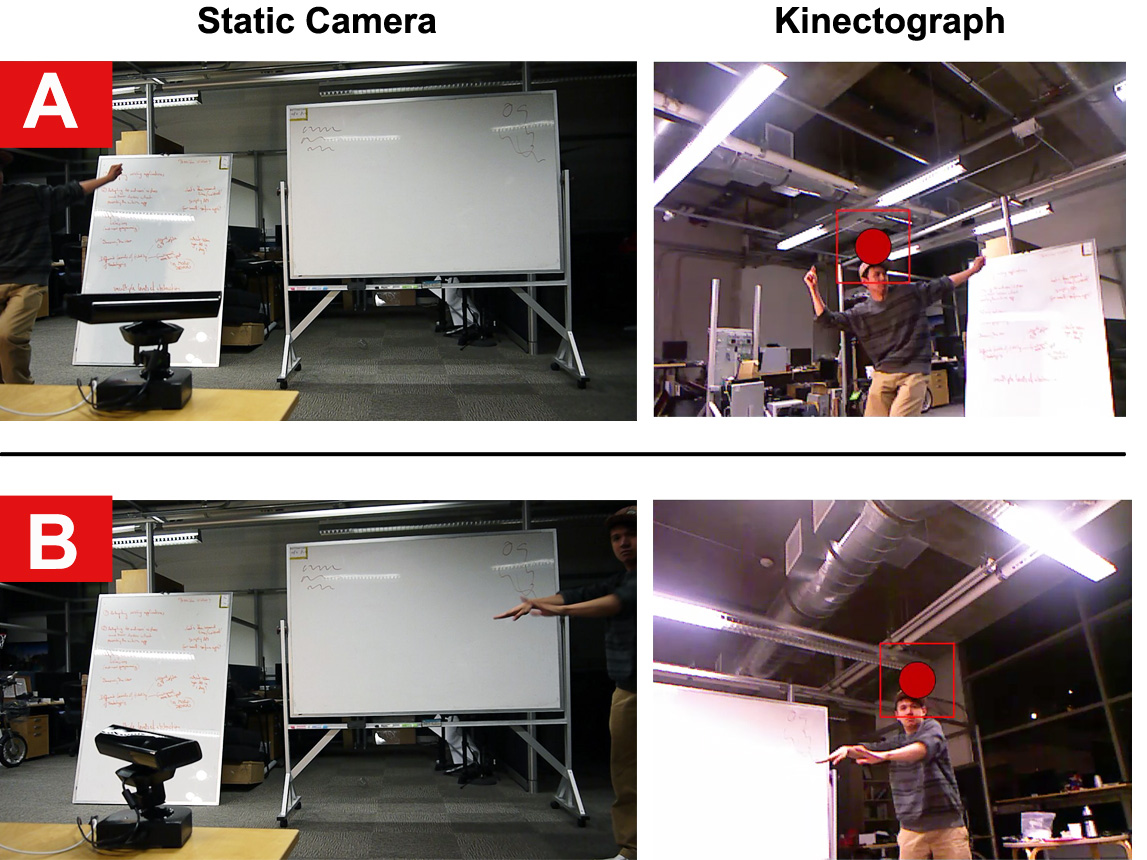
\includegraphics[width=0.5\columnwidth]{\kinectograph/fig/OurExamples-2x2}
    \caption{Examples of camera views captured by a static camera and Kinectograph at two specific moments in time.}
    \label{fig:kinectograph_dance}
\end{figure}

Table~\ref{tab:kinectograph_first_tasks} shows details of the four tasks and analysis of the recorded videos. We categorized physical activities into three movement types: \emph{Continuous} (user continuously moves around), \emph{Periodic} (user moves, stays, and moves again periodically), and \emph{Occasional} (no clear motion pattern was observed).
%
There were two Continuous and two Periodic tasks that participants designed. The moving range was about 15 feet in a home environment, and participants set the static camera about 8 feet away from the center of their workspace. Participants chose this distance to avoid out-of-frame problems with the static camera: \iquote{The distance was chosen so that all of the activity could be captured} (P4). Kinectograph was placed 6 feet away on a tabletop by the experimenters to capture the participant's whole body. Participants were allowed to adjust the camera angle via our tablet UI before recording the demonstration.

All the participants chose to track their heads, but note
that their activities involved frequent turning where
pure face recognition might fail. Participants did not
change this setting during the performance, although
they were allowed to. P2 changed to the manual mode
for testing, switched back, and then continued the
activity. The average video length is one and half
minutes long.

All the participants agreed or strongly agreed that
Kinectograph captured what they intended to show,
while only half of them agreed that the static camera
captured as expected. The main reason was the
limited static camera angle; in three tasks, participants
moved out of the static camera view more than once. Figure~\ref{fig:kinectograph_dance} shows two examples where our system
captured what the static camera missed. It was worth
noting that although P3 had set and confirmed the
viewpoint before recording, he was not aware that he
shortly but frequently (9 times) went over the
boundaries when he was demonstrating. He explained
that he preferred using Kinectograph because it \iquote{kept
us in the center of view no matter how we moved
around.} This shows that Kinectograph successfully
ensured the activities would be captured and therefore
enabled users to focus on their tasks.

\subsection{Study 3: Self-Recording Activities}

Finally, we conducted a study to measure whether users could film an entire demonstration video using Kinectograph with minimal aid.
%
We recruited seven participants (3 male and 4 females, ages 20-33) from a university to record multi-step tutorials in a lab environment. Four had filmed a video before but only one had filmed a video without the assistance of others. Each participant was compensated with a \$10 giftcard. Each session lasted about 30 minutes long.
% Note that this experiment was run using a previous prototype of the Kinectograph base, which did not utilize the motors provided by the Kubi.
%\pc{describe the settings and put the figure here}
%14-16 feet by 12-14 feet area
Below we describe the procedure of this study:
\subsubTitleBold{Introduction (5 minutes)} Participants first went through an online documentation to learn the Kinectograph features. %with a demo video

\subsubTitleBold{Training (10 minutes)} Experimenters guided participants through a series of interactions highlighting each of our core features. Participants were asked to operate each feature through our tablet UI with the support of experimenters.

\subsubTitleBold{Testing (5 minutes)} We asked participants to film a basketball tutorial using Kinectograph. They were asked to introduce actions including passing, catching, and tossing a basketball. Participants acted as both an actor and a director, i.e., they fully controlled the camera and performed the demonstrations without any assistance. A series of nine subtasks were designed for participants to exercise the following features: manual mode (pan/tilt), tracking mode (to track single and multiple body joints), and zooming. In particular, one of the subtasks involved two users in the view. Experimenter walked in the view for passing the ball when participant invited. To help participants understand these activities, we provided a storyboard with high level instructions for filming (e.g., ``zoom into your face'', ``pan to the basketball'', or ``track your head and walk around'') without explicitly listing which Kinectograph feature to use. During the recording, we captured Kinectograph's rendered video view.

\subsubTitleBold{Questionnaire and Debrief (10 minutes)} Finally, we asked participants to watch the recorded video in full and answer a questionnaire, regarding the ease of use of our interface and open-ended questions. We monitored the number of attempts it took to complete each filming task of the tutorials.

\subsubsection{Results}
All of the 7 participants successfully created a self-directed tutorial using our system. No users failed to complete any of the 9 subtasks. Each participant reattempted at most 2 subtasks, mostly to reselect a zoom area. The average video length was 3.5 minutes. Overall, participants rated the ease of use of the system as $\mu=4.1$ on the 5-point Likert scale.
%
All participants were able to manually pan and tilt the camera by swiping as intended. Participants stated that this was easy to control with the UI ($\mu=3.6$ , $\sigma = 1.0$). They also successfully enabled the tracking mode and had Kinectograph track their head and hands. Participants stated it was easy to enable tracking ($\mu=4, \sigma=1.3$ ) and rated their satisfaction with the system performance as $\mu=4, \sigma=0.8$.  Participants stated that \iquote{It was easy to select a body part of choice} (P6), and that \iquote{ (...Kinectograph) could center the screen very well, and accurately tracked the person} (P7). Four users specifically mentioned that zooming was one of the features that worked well. Participants were satisfied with their video recording ($\mu=4.1$, $\sigma=0.7$).

We also learned some important shortcomings from the study. Notably, the pan-tilt motors that our previous Kinectograph prototype uses is under-dimensioned, which leads to oscillation (camera shake) when Kinectograph performs large amplitude pan movements. This is less noticeable at further distances, but becomes especially problematic when the users zooms in on small regions. Learning this effect, we have removed this issue with our current use of Kubi's servos, which provide smooth motor control.

Latency in video streaming to the tablet device hampered usability. As P4 stated: \iquote{The lag made it difficult for me to move the kinectograph smoothly [during manual control]}.
%
% Tracking multiple actors remained somewhat difficult (a confederate joined for a ball passing task). P1 stated \iquote{Shortcomings were only really with multiple people in the demo, and the limitations of the viewing angle of the Kinect itself.}
%
Participants also suggested alternative control modes other than a tablet while engaged in bi-manual tasks: \iquote{Certain demos require the use of multiple hands, meaning that I can't carry the iPad during the demo if i wanted to change the point of focus on my body. It would be nice if there were gestures i could do to switch the point(s) of focus without having to use the iPad.} We found this concept interesting and plan to explore in future work.

% \begin{figure}[t]
% \centering
% 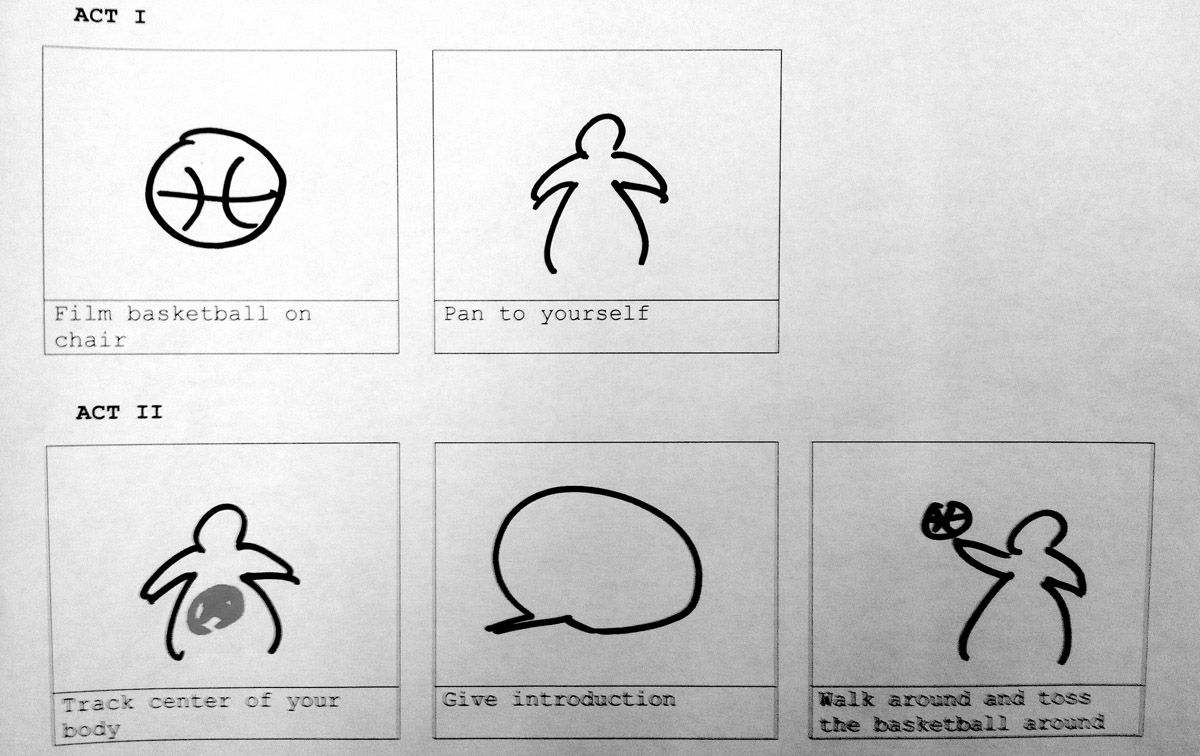
\includegraphics[width=1.0\columnwidth]{userStudy}
% \caption{We presented participants in the second procedure with a storyboard of actions they should perform.}
% \label{fig:storyboard}
% \end{figure}
% In aggregate, our evaluation suggests that Kinectograph system is capable of being used to create tutorial videos but also points the way for future work. Future work comprises improvements to live video streaming, better support of multiple users (i.e. using voice commands or gesture cues to control), and using kinectic info and zoom as meta data for playback.
% and more Tablet UI features, such as picture in picture view and more boxes on the UI to provide further feedback to the user.
